% !TEX root = cto-framework-book.tex

\documentclass[a4paper]{book}

\usepackage[english]{babel} % Language support
\usepackage[T1]{fontenc}    % Proper font encoding
\usepackage{lmodern}        % Better font rendering
% \usepackage{mlmodern}

\usepackage{fontspec}
\setmainfont{IBM Plex Sans}

\usepackage{graphicx} % Required for inserting images
\graphicspath{{images/}{../images/}}

\usepackage{sectsty}
\chapterfont{\color{secondarycolor}}

\usepackage{tikz}          % For creating graphical elements and colors
\usepackage{tikz-3dplot} 

\newcommand{\booktitle}{CTO Framework}
\newcommand{\bookauthor}{Santiago Lizardo}
\newcommand{\booklicence}{Creative Commons Attribution 4.0 International (CC BY 4.0)}

\usepackage[dvipsnames]{xcolor}

\definecolor{primarycolor}{HTML}{CB54F2}
\definecolor{secondarycolor}{HTML}{2A64B3}
\definecolor{color1}{HTML}{CB54F2}
\definecolor{color2}{HTML}{2A64B3}
\definecolor{color3}{HTML}{377E8C}
\definecolor{color4}{HTML}{421869}
\definecolor{color5}{HTML}{A9F2FB}
\definecolor{color6}{HTML}{040505}


\usepackage{amsmath} % For environment equation

\usepackage{afterpage}

\usepackage{geometry}
\usepackage{array}
\usepackage{fontawesome5}
\usepackage{longtable}

\usepackage{imakeidx}
\makeindex[intoc]

\usepackage{tcolorbox}

\newtcolorbox{tipbox}{
    colback=color1!10, colframe=color3!50!black,  % Background and border colors
    coltitle=color5, fonttitle=\bfseries,         % Title font and color
    title={\faLightbulb\ Tip},
    sharp corners=south                         % Rounded corners only at top
}

\usepackage{listings}
\lstdefinestyle{pythonstyle}{
    language=Python,
    backgroundcolor=\color{gray!10},   % Choose the background color
    basicstyle=\ttfamily\small,          % Choose the font and size
    keywordstyle=\color{blue},            % Keywords color
    commentstyle=\color{green},           % Comments color
    stringstyle=\color{red},              % Strings color
    numbers=left,                        % Line numbers on the left
    numberstyle=\tiny\color{gray},        % Line numbers style
    stepnumber=1,                        % Line numbers step
    numbersep=5pt,                       % Distance from line numbers to code
    tabsize=4,                           % Tab size
    showspaces=false,                    % Show spaces in code
    showstringspaces=false,              % Show spaces in strings
    showtabs=false,                      % Show tabs in code
    frame=single,                        % Frame around code
    rulecolor=\color{black},             % Frame color
    breaklines=true,                     % Enable automatic line breaking
    breakatwhitespace=true,              % Break lines at whitespace (optional)
}

\usepackage{hyperref}
\hypersetup{
    colorlinks=true, %set true if you want colored links
    linktoc=all,     %set to all if you want both sections and subsections linked
    linkcolor=blue,  %choose some color if you want links to stand out
    pdftitle = {CTO Framework},
    pdfauthor = {\bookauthor},
    pdfkeywords = {leadership, technology, innovation, management},
    pdfsubject = {Technology leadership},
}

\usepackage{pgfplots}
\pgfplotsset{compat=1.18}
\usepackage{pgfmath}
\pgfmathdeclarefunction{gamma}{1}{%
    \pgfmathparse{exp(-0.5772156649015328606*(#1-1))*
        sqrt(2*3.1415926535897932384626433832795*(#1-1))*
        ((#1-1)/2.7182818284590452353602874713527)^((#1-1))}%
}

\usepackage{fancyhdr}

\pagestyle{fancy} % Enable fancy headers/footers
\fancyhf{} % Clear all headers and footers

% Define header (only on right-hand pages)
\fancyhead[RO]{\rightmark}

% Define footer (only on right-hand pages)
\fancyfoot[RO]{\rule{\textwidth}{0.4pt} \\ \thepage}

% Ensure chapter names appear correctly
\renewcommand{\chaptermark}[1]{\markright{\thechapter\quad #1}}

% Ensure the first page of a chapter does not have headers
\fancypagestyle{plain}{
    \fancyhf{}
    \renewcommand{\headrulewidth}{0pt} % Remove header rule
    \fancyfoot[RO]{\rule{\textwidth}{0.4pt} \\ \thepage}
}
\input{git-info}

\title{\booktitle}
\author{\bookauthor}
\date{\GitTag\ - \the\year{}}

\begin{document}

\frontmatter

\pagestyle{empty}


\begin{tikzpicture}[remember picture, overlay]
    % Background gradient (dark sky to neon blue horizon)
    \shade[top color=black, bottom color=blue!60!black]
    (current page.south west) rectangle (current page.north east);

    % Horizon Glow
    \draw [white, opacity=0.5] (-5,3) -- (5,3);
    \fill [blue!70!black] (-5,2.8) rectangle (5,3);

    % 3D Perspective Grid
    \begin{scope}[canvas is xy plane at z=0, transform shape]
        \foreach \x in {-10,-9,...,10} {
                \draw[magenta!80] (\x,-1) -- (0,4);
            }
        \foreach \y in {-1,0,...,3} {
                \draw[magenta!80] (-10,\y) -- (10,\y);
            }
    \end{scope}

    % Book Title
    \node[text=white, font=\bfseries\Huge] at (current page.north)
    [yshift=-2cm] {CTO Framework};

    % Subtitle
    \node[text=white, font=\LARGE] at (current page.north)
    [yshift=-4cm] {A Strategic Guide for Tech Leaders};

    % Author Name
    \node[text=white, font=\Large] at (current page.south)
    [yshift=2cm] {By Santiago Lizardo | \GitTag\ - \the\year{}};
\end{tikzpicture}
\newpage % Or \cleardoublepage

\begin{flushleft}
    \textbf{\Large \booktitle}

    \vspace{1cm}

    Revision: \GitTag\\
    Last Updated: \today \\
    % ISBN: XXX-X-XXX-XXXXX-X \\
    License: \booklicence

    \vspace{1cm}

    Author: \bookauthor\\
    Contact: \url{info@ctoframework.com}

\end{flushleft}

\newpage
\tableofcontents

\mainmatter
\pagestyle{fancy}


\begin{center}
    \thispagestyle{empty}
    \vspace*{\fill}
    Dedicated to my family, for their unconditional support.
    \vspace*{\fill}
\end{center}

\chapter{The CTO's Playbook}

\section{What This Book Covers}

The role of a Chief Technology Officer (CTO) is one of the most dynamic and demanding positions in any organization. It sits at the intersection of technology, business strategy, and leadership, requiring a unique blend of technical acumen, people management skills, and strategic foresight. However, there is no single blueprint for success-every company is different, and every CTO must adapt to their specific context.

This book provides a structured framework to help CTOs navigate their responsibilities effectively. It is designed to be a practical guide, offering insights and actionable strategies across four key areas that define the role: People, Processes, Product, and Technology.

\subsection{People: Building and Leading Teams}

A CTO's success is directly tied to the quality of their team. Hiring, developing, and retaining the right talent is as crucial as making sound technical decisions. This section delves into leadership strategies, culture-building, and effective organizational structures that foster high-performance engineering teams. It explores challenges such as scaling teams, managing remote workforces, and aligning technical talent with business objectives.

\subsection{Processes: Optimizing for Efficiency}

Technology teams thrive on clarity and efficiency. Without the right processes in place, even the most talented engineers can struggle to deliver value. This section focuses on operational excellence, covering areas such as agile methodologies, DevOps practices, release management, and stakeholder communication. The goal is to equip CTOs with strategies to streamline workflows, enhance collaboration, and ensure that the technology function operates smoothly.

\subsection{Product: Strategy and Execution}

A CTO must have a deep understanding of the company's product vision and how technology enables it. This section examines how to align technical roadmaps with business goals, work effectively with product teams, and make decisions that balance innovation with pragmatism. Topics include prioritization frameworks, scaling products, and managing technical debt while keeping a focus on delivering customer value.

\subsection{Technology: Architecture and Scalability}

While leadership and strategy are essential, a CTO is ultimately responsible for the organization's technical foundations. This section explores core technical topics, from choosing the right architecture and tech stack to ensuring scalability and security. It provides guidance on making long-term architectural decisions, adopting emerging technologies, and mitigating risks associated with technical evolution.

By addressing these four areas comprehensively, this book aims to serve as a playbook for CTOs at any stage of their journey-whether they are stepping into the role for the first time, leading a startup through hypergrowth, or managing technology at a large-scale enterprise.

\section{How to Use This Framework}

This book is not meant to be read once and shelved. Instead, it is designed as a practical reference that you can return to as new challenges arise. The framework is modular, allowing you to focus on specific areas depending on your current priorities.

If you are building your leadership skills, start with the People section. If your team struggles with inefficiencies or bottlenecks, jump to the Processes section. If aligning technology with business strategy is your challenge, the Product section will offer valuable insights. And if you need to make key architectural decisions, the Technology section provides guidance on best practices for scalability and reliability.

Throughout the book, you will find real-world examples, decision-making frameworks, and actionable takeaways to apply in your role. These are drawn from a combination of personal experiences, industry best practices, and insights from seasoned technology leaders.

Additionally, while this book provides guidance, it does not prescribe a one-size-fits-all approach. Every company has a unique culture, market, and technology stack. Use this framework as a foundation, but adapt it to fit your organization's specific needs.

A CTO's role is ever-evolving. What works today may not be relevant in a year as technologies, teams, and business landscapes shift. The key to success is continuous learning and adaptation. Consider this book a toolkit to help you navigate the complexities of the role, make informed decisions, and ultimately drive technological and business success.




\chapter{People: Building and Leading Teams}
\section{Defining the CTO's Role}
\section{Hiring and Retaining Top Talent}
\subsection{Recruitment Strategies}
\subsection{Interviewing and Selection}
\subsection{Onboarding and Growth}
\section{Creating a High-Performance Culture}
\subsection{Fostering Collaboration}
\subsection{Psychological Safety and Accountability}
\subsection{Diversity, Equity, and Inclusion}
\section{Leadership and Communication}
\subsection{Managing Up, Down, and Sideways}
\subsection{Aligning Vision with Execution}
\subsection{Handling Difficult Conversations}
\chapter{Processes: Optimizing for Efficiency}
\section{Agile, DevOps, and Beyond}
\subsection{Choosing the Right Methodology}
\subsection{Continuous Integration and Deployment}
\subsection{Reducing Bottlenecks}
\section{Effective Roadmaps and Prioritization}
\subsection{Balancing Short-Term and Long-Term Goals}
\subsection{Stakeholder Management}
\section{Governance, Risk, and Compliance}
\subsection{Regulatory Considerations}
\subsection{Security and Data Privacy}
\subsection{Ethical Considerations in Tech}
\chapter{Product: Strategy and Execution}


\section{Product and Business Alignment}

The symbiotic relationship between product strategy and overarching business objectives is paramount for the success of any technology-driven organization. The \gls{CTO}, positioned at the intersection of technology and business, plays a pivotal role in ensuring this alignment. This section delves into the critical aspects of understanding business objectives and defining the \gls{CTO}'s influence within product decisions.

\subsection{Understanding Business Objectives}
Aligning technology with business objectives is not merely a desirable outcome but a fundamental responsibility of a \gls{CTO}. This necessitates a profound and nuanced understanding of the company's overarching goals, its strategic market positioning, and the ever-evolving needs and expectations of its customer base. Without this deep comprehension, technological endeavors risk becoming detached from the core value proposition of the business, leading to misallocation of resources and ultimately hindering growth.

\subsubsection{Revenue and Growth Targets}
A primary driver for any business is the generation of revenue and the achievement of sustainable growth. Technology decisions must be intrinsically linked to the company's revenue models. Whether the business operates on a subscription-based (\textit{e.g.}, \gls{SaaS}), transactional (\textit{e.g.}, e-commerce), or advertising-driven model, the technological infrastructure and product development roadmap must actively support and enhance these mechanisms. For instance, a subscription-based company might prioritize features that increase user retention and upsell opportunities, while an e-commerce platform would focus on scalability, secure payment processing, and personalized product recommendations. Understanding the specific revenue targets and growth aspirations provides a crucial lens through which all technology decisions should be evaluated. The \gls{CTO} must ensure that the technological architecture can scale to accommodate projected growth and that product features are designed to directly contribute to revenue generation.

\subsubsection{Market Positioning and Competitive Advantage}
Identifying the company's current and desired position within the competitive landscape is crucial. Understanding where the company stands in comparison to its rivals, their strengths, and their weaknesses allows the \gls{CTO} to leverage technology as a strategic differentiator. Technology can be a powerful tool for creating a sustainable competitive advantage\footnote{Porter, M. E. (1985). \textit{Competitive Advantage: Creating and Sustaining Superior Performance}. Free Press.} by enabling unique product features, optimizing operational efficiency, or delivering superior customer experiences. The \gls{CTO} must actively participate in strategic discussions to understand the desired market positioning and then translate this into a technological vision that supports and amplifies the company's competitive edge. This might involve investing in emerging technologies, developing proprietary algorithms, or building a highly scalable and resilient infrastructure that outperforms competitors.

\subsubsection{Customer Experience}
In today's customer-centric environment, the experience a company provides is often as important as the product itself. Ensuring that product development aligns with the goal of improving \gls{UX} and engagement is paramount. Technology plays a direct role in shaping this experience, from the intuitiveness of the user interface to the responsiveness of the platform and the quality of customer support. The \gls{CTO} must champion a customer-centric approach within the technology organization, ensuring that product teams prioritize user needs and incorporate feedback into the development process. This involves implementing robust user research methodologies, employing data analytics to understand user behavior, and fostering a culture of continuous improvement focused on enhancing the overall customer journey.

\subsubsection{Regulatory and Compliance Requirements}
Navigating the complex landscape of industry standards and compliance constraints is an increasingly critical aspect of product development. Depending on the industry and geographical location, companies may be subject to a wide range of regulations concerning data privacy, security, accessibility, and industry-specific standards (e.g., HIPAA in healthcare, GDPR in Europe, PCI DSS for payment processing). The \gls{CTO} bears the responsibility of ensuring that all product development efforts adhere to these requirements from the outset. Failure to comply can result in significant financial penalties, reputational damage, and legal repercussions. This necessitates a proactive approach to understanding and implementing relevant regulations, integrating compliance considerations into the software development lifecycle, and maintaining ongoing vigilance to adapt to evolving legal frameworks.

\subsection{Defining the CTO's Role in Product Decisions}
The \gls{CTO}'s involvement in product decisions transcends mere technical implementation; it requires a delicate balance of technical leadership and strategic product influence. The specific nature and extent of this role can vary significantly depending on factors such as company size, organizational structure, and the company's stage of growth. However, certain core responsibilities generally fall within the purview of the \gls{CTO} in shaping the product landscape.

\subsubsection{Technology Vision and Roadmap}
A fundamental aspect of the \gls{CTO}'s role is the articulation and maintenance of a clear technology vision and roadmap that directly supports the overarching business goals. This involves anticipating future technological trends, evaluating their potential impact on the business, and strategically planning the evolution of the company's technology stack and infrastructure. The \gls{CTO} must ensure that the proposed technical solutions are not only feasible and scalable but also aligned with the long-term strategic direction of the product and the business as a whole. This requires a deep understanding of both the technical possibilities and the business imperatives, enabling the \gls{CTO} to guide technology investments and development efforts in a way that maximizes their strategic impact.

\subsubsection{Collaboration with Product Teams}
Effective collaboration with Product Management\index{Product Management} is crucial for aligning technical capabilities with market needs and customer demands. The \gls{CTO} and their team must work in close partnership with product managers to understand the market landscape, identify unmet customer needs, and translate these into viable product features and functionalities. This collaborative process ensures that technical feasibility is considered early in the product development lifecycle, preventing the pursuit of technically challenging or unscalable ideas. Furthermore, it allows for the exploration of innovative technical solutions that can provide a competitive edge and enhance the value proposition of the product. Regular communication, shared understanding of priorities, and a spirit of mutual respect are essential for fostering a productive and impactful partnership between technology and product teams.

\subsubsection{Risk Management}
Product decisions inherently involve a degree of technical risk. The \gls{CTO} plays a critical role in identifying, assessing, and mitigating these risks early in the development process. This includes evaluating the feasibility of proposed technical solutions, identifying potential security vulnerabilities, assessing the scalability and reliability of the chosen technologies, and anticipating potential integration challenges. By proactively addressing these risks, the \gls{CTO} helps to ensure the successful and timely delivery of high-quality products. This involves implementing robust testing strategies, establishing clear architectural guidelines, and fostering a culture of security and quality within the engineering organization.

\subsubsection{Stakeholder Communication}
The \gls{CTO} often serves as a crucial bridge between the technical complexities of product development and the business-oriented perspectives of executives and investors. The ability to translate technical constraints, opportunities, and trade-offs into clear and concise business language is essential for effective communication and decision-making at the highest levels of the organization. This involves explaining the strategic implications of technical choices, articulating the potential \gls{ROI} of technology investments, and providing insights into the technological landscape that can inform business strategy. The \gls{CTO} must be adept at tailoring their communication style to different audiences, ensuring that both technical and non-technical stakeholders have a clear understanding of the technological aspects of the product strategy.

\section{Integrating Technology into Product Strategy}

The integration of technology considerations into the overarching product strategy is not a separate activity but rather an intrinsic element of successful product development. The \gls{CTO} plays a key role in ensuring that technology is not viewed as a mere enabler but as a strategic driver of product innovation and differentiation.

\subsection{Technology as a Differentiator}
In today's competitive landscape, technology can be a significant differentiator, allowing companies to offer unique product features, superior performance, and enhanced user experiences. The \gls{CTO} must actively explore and champion the adoption of cutting-edge technologies that can provide a competitive edge. This might involve leveraging artificial intelligence and machine learning to personalize user experiences, utilizing blockchain technology for enhanced security and transparency, or adopting serverless architectures for improved scalability and cost-efficiency. By strategically integrating such technologies into the product roadmap, the \gls{CTO} can help the company stand out from the competition and attract and retain customers.

\subsection{Scalability and Reliability}
As products grow in popularity and usage, the underlying technology infrastructure must be able to scale seamlessly to handle increased demand while maintaining reliability and performance. The \gls{CTO} is responsible for ensuring that the product architecture is designed with scalability and resilience in mind. This involves making strategic decisions about infrastructure choices, database technologies, and deployment strategies that can accommodate future growth and minimize the risk of downtime or performance degradation. A scalable and reliable technology platform is crucial for maintaining customer satisfaction and supporting the long-term success of the product.

\subsection{Innovation and Experimentation}
Fostering a culture of innovation and experimentation within the technology organization is essential for driving product evolution. The \gls{CTO} should encourage teams to explore new technologies, experiment with different approaches, and rapidly iterate on product features. This might involve setting aside dedicated time for research and development, implementing agile development methodologies, and creating a safe environment for experimentation and learning from failures. By embracing innovation, the company can continuously improve its products, adapt to changing market conditions, and stay ahead of the competition.

\subsection{Data-Driven Product Development}
Data plays an increasingly important role in informing product decisions. The \gls{CTO} must ensure that the necessary infrastructure and processes are in place to collect, analyze, and interpret relevant data insights. This data can provide valuable information about user behavior, feature usage, performance metrics, and market trends, which can then be used to guide product development efforts and prioritize features that deliver the most value to users and the business. By fostering a data-driven culture, the \gls{CTO} can help ensure that product decisions are based on evidence rather than assumptions, leading to more effective and impactful outcomes.


\section{Balancing Innovation and Execution}

\subsection{Managing Technical Debt}
Technical debt is an inevitable part of software development but must be actively managed to ensure sustainable growth.

\begin{table}[h]
    \centering
    \begin{tabular}{|c|c|}
        \hline
        \textbf{Type of Technical Debt} & \textbf{Impact}                                   \\
        \hline
        Intentional                     & Short-term gains, long-term costs                 \\
        \hline
        Accidental                      & Results from poor decisions or lack of knowledge  \\
        \hline
        Environmental                   & Arises due to technology changes and system aging \\
        \hline
    \end{tabular}
    \caption{Types of Technical Debt}
\end{table}

Key strategies for managing technical debt include:

\begin{itemize}
    \item Regular refactoring and addressing debt incrementally.
    \item Prioritizing high-impact debt resolution.
    \item Educating stakeholders on long-term costs of accumulated debt.
\end{itemize}

\subsection{Evaluating Build vs. Buy Decisions}
A CTO must decide when to build custom solutions and when to leverage third-party tools. Considerations include:

\begin{itemize}
    \item \textbf{Cost:} Initial development vs. long-term maintenance expenses.
    \item \textbf{Time-to-Market:} Off-the-shelf solutions may accelerate launch.
    \item \textbf{Customization Needs:} Whether existing solutions meet specific business requirements.
    \item \textbf{Vendor Lock-in:} Dependencies and risks associated with third-party providers.
\end{itemize}

\section{Data-Driven Decision Making}

\subsection{Metrics That Matter}
Choosing the right metrics is critical to measuring success. Common product and technical metrics include:

\begin{itemize}
    \item \textbf{North Star Metric:} A single metric representing long-term company success.
    \item \textbf{Customer Retention Rate:} Indicates long-term product value.
    \item \textbf{Technical Performance:} System uptime, response times, and error rates.
    \item \textbf{Development Velocity:} Sprint completion rates and cycle times.
\end{itemize}

\subsection{Experimentation and Validation}

In an era where technology evolves rapidly, a Chief Technology Officer (CTO) must foster a culture of experimentation and validation to drive innovation and make informed decisions. This approach ensures that strategic initiatives are backed by data, reducing the risk of costly missteps and enabling continuous improvement.

\subsubsection{The Role of Experimentation in Technology Leadership}
Experimentation in technology leadership involves systematically testing new ideas, features, and products before full-scale implementation. A structured approach to experimentation enables organisations to measure real user impact, validate assumptions, and refine strategies based on empirical evidence.

A CTO should embed experimentation into the company’s technology strategy, ensuring that the organisation remains agile, user-focused, and competitive. Effective experimentation involves defining hypotheses, running controlled tests, and analysing results to guide product development and business decisions.

\subsubsection{Key Components of an Experimentation Culture}
To successfully integrate experimentation into an organisation, a CTO should focus on the following key components:

\begin{itemize}
    \item \textbf{Hypothesis-Driven Development:} Every experiment should begin with a well-defined hypothesis. This ensures clarity of purpose and measurable outcomes. For example, "If we reduce the checkout process from three steps to one, we expect a 15\% increase in conversion rates."
    \item \textbf{Controlled Experiments:} Running controlled A/B tests or multivariate experiments helps measure the direct impact of a change. This involves dividing users into test and control groups to compare outcomes.
    \item \textbf{Iterative Development:} Rapid iterations based on experiment outcomes enable continuous improvement. Instead of large, risky deployments, small incremental changes allow for quick adaptation.
    \item \textbf{Data-Driven Decision Making:} Results from experiments should guide product and business strategies. This requires robust data collection, analysis, and interpretation to extract actionable insights.
    \item \textbf{User Feedback Integration:} Direct input from users through surveys, usability testing, and customer support interactions can provide qualitative insights to complement quantitative data.
\end{itemize}

\subsubsection{Framework for Experimentation and Validation}
A well-structured framework ensures that experimentation efforts are methodical and aligned with organisational goals. Below is a suggested framework:

\begin{table}[h]
    \centering
    \begin{tabular}{|l|l|}
        \hline
        \textbf{Phase}       & \textbf{Description}                                                                                  \\
        \hline
        Identify Problem     & Define the business or user problem to be addressed.                                                  \\
        \hline
        Formulate Hypothesis & Develop a testable statement predicting the outcome of the change.                                    \\
        \hline
        Design Experiment    & Determine experiment type (A/B test, multivariate test, feature flagging) and define success metrics. \\
        \hline
        Run Experiment       & Deploy the experiment to a sample user base while monitoring key metrics.                             \\
        \hline
        Analyse Results      & Assess whether the hypothesis was supported by the data.                                              \\
        \hline
        Implement or Iterate & Roll out successful changes or refine and retest unsuccessful ones.                                   \\
        \hline
    \end{tabular}
    \caption{Experimentation and Validation Framework}
\end{table}

\subsubsection{Examples of Experimentation in Practice}
Many leading technology companies leverage experimentation to drive innovation and validate strategic decisions:

\begin{itemize}
    \item \textbf{Google:} The company is known for conducting thousands of A/B tests annually to refine its search algorithms, UI changes, and product offerings.
    \item \textbf{Netflix:} Uses extensive experimentation to optimise recommendation algorithms, interface changes, and content engagement strategies.
    \item \textbf{Amazon:} Implements controlled tests to enhance user experience, pricing strategies, and conversion rates on its e-commerce platform.
\end{itemize}

\subsubsection{Challenges in Experimentation and How to Overcome Them}
While experimentation is a powerful approach, it comes with challenges that a CTO must address:

\begin{itemize}
    \item \textbf{Experimentation Fatigue:} Running too many tests simultaneously can overwhelm teams and users. Prioritising high-impact experiments mitigates this risk.
    \item \textbf{Statistical Validity:} Small sample sizes or biased test groups can lead to misleading conclusions. Ensuring statistical rigor in experiment design is crucial.
    \item \textbf{Cultural Resistance:} Teams may be resistant to experimentation due to fear of failure. Fostering a "fail fast, learn faster" mindset encourages innovation.
\end{itemize}

\subsubsection{Conclusion}
A CTO’s role in fostering an experimentation culture is critical to an organisation’s success. By implementing a structured framework, leveraging data-driven decision-making, and learning from industry best practices, companies can drive continuous improvement and maintain a competitive edge.

Encouraging a mindset of "test, learn, and iterate" ensures that technology teams build products that truly meet user needs while minimising risks associated with large-scale deployments. As technology landscapes evolve, experimentation remains a cornerstone of agile and responsive leadership.

\subsubsection{References}
\begin{itemize}
    \item Kohavi, R., Longbotham, R., Sommerfield, D., \& Henne, R. (2009). \textit{Controlled experiments on the web: survey and practical guide}. Data Mining and Knowledge Discovery.
    \item Thomke, S. (2020). \textit{Experimentation Works: The Surprising Power of Business Experiments}. Harvard Business Review Press.
    \item Netflix Tech Blog. (2022). \textit{Improving recommendations through experimentation}. Retrieved from \url{https://netflixtechblog.com}
\end{itemize}



\subsection{Scaling Successfully}
Ensuring a product scales effectively requires technical foresight and architectural planning. Key considerations include:

\begin{itemize}
    \item Designing for horizontal and vertical scalability.
    \item Leveraging cloud infrastructure for elasticity.
    \item Optimizing database performance for high-load scenarios.
    \item Implementing effective caching strategies.
\end{itemize}

Scalability is not just a technical challenge but a business enabler, ensuring that growth does not outpace infrastructure capabilities.

\chapter{Technology: Architecture and Scalability}

\section{Defining a Scalable Tech Strategy}

A scalable technology strategy is foundational to any growing organization. A well-architected strategy ensures that the system can handle increased loads, adapt to changing business requirements, and maintain efficiency as the company evolves. This section explores key elements such as technology selection, evaluation, and future-proofing systems.

\subsection{Technology Selection and Evaluation}

Choosing the right technology stack is critical for long-term scalability and maintainability. The decision-making process should be systematic, taking into account technical and business factors.

\textbf{Key Factors in Technology Selection:}
\begin{itemize}
    \item \textbf{Performance:} Ensuring the selected technology meets required latency and throughput demands.
    \item \textbf{Scalability:} Assessing how well the technology scales horizontally and vertically.
    \item \textbf{Community and Support:} Evaluating the ecosystem, documentation, and vendor support.
    \item \textbf{Security:} Ensuring compliance with industry standards and security best practices \index{security}.
    \item \textbf{Total Cost of Ownership (TCO):} Considering licensing, operational, and maintenance costs.
\end{itemize}

A comparison table can help in technology evaluation:

\begin{table}[ht]
    \centering
    \begin{tabular}{|l|c|c|c|}
        \hline
        \textbf{Criteria} & \textbf{Technology A} & \textbf{Technology B} & \textbf{Technology C} \\
        \hline
        Performance       & High                  & Medium                & Low                   \\
        Scalability       & High                  & High                  & Medium                \\
        Community Support & Strong                & Moderate              & Weak                  \\
        Cost              & Low                   & High                  & Medium                \\
        \hline
    \end{tabular}
    \caption{Technology Selection Matrix}
    \label{tab:tech_selection}
\end{table}

\subsection{Future-Proofing Systems}

Future-proofing technology ensures longevity and adaptability. Some key principles include:

\begin{itemize}
    \item \textbf{Modular Architecture:} Designing systems with clear separation of concerns (e.g., microservices\index{microservices}).
    \item \textbf{Loose Coupling:} Ensuring components communicate via well-defined APIs to minimize dependencies.
    \item \textbf{Backward Compatibility:} Designing systems that support legacy data and integrations.
    \item \textbf{Observability:} Embedding monitoring and logging for proactive issue resolution.
\end{itemize}

\section{Engineering Best Practices}

\subsection{Code Quality and Standards}

Code quality is essential for maintainability and collaboration. Best practices include:

\begin{itemize}
    \item \textbf{Consistent Coding Style:} Using linters and formatters (e.g., Prettier, ESLint).
    \item \textbf{Code Reviews:} Implementing peer reviews to catch bugs early.
    \item \textbf{Documentation:} Maintaining inline and API documentation.
\end{itemize}

\begin{tipbox}
    \textbf{Do not reinvent the wheel:} Programming languages and frameworks have established best practices. Follow them to ensure maintainability and readability.\\
    \\
    \textbf{TypeScript examples:}
    \begin{itemize}
        \item \url{https://docs.aws.amazon.com/prescriptive-guidance/latest/best-practices-cdk-typescript-iac/typescript-best-practices.html}
        \item \url{https://google.github.io/styleguide/tsguide.html}
    \end{itemize}
\end{tipbox}

\subsection{Testing and Automation}

Automated testing improves reliability and efficiency.

\begin{itemize}
    \item \textbf{Unit Tests:} Validating individual components.
    \item \textbf{Integration Tests:} Ensuring components work together.
    \item \textbf{Continuous Integration (CI):} Automating test execution on every commit.
\end{itemize}

\subsection{Security by Design}

Security should be embedded from the start.

\begin{itemize}
    \item \textbf{Threat Modeling:} Identifying potential vulnerabilities.
    \item \textbf{Least Privilege Principle:} Granting only necessary access.
    \item \textbf{Regular Audits:} Conducting security reviews and penetration testing.
\end{itemize}

\section{Infrastructure and Operations}

\subsection{Cloud vs. On-Premise Considerations}

Choosing between cloud\index{cloud} and on-premise\index{on-premise} solutions involves several trade-offs:

\begin{itemize}
    \item \textbf{Scalability:} Cloud solutions offer elastic scaling, whereas on-premise requires capacity planning.
    \item \textbf{Cost:} Cloud follows an OPEX model, while on-premise is typically CAPEX.
    \item \textbf{Control:} On-premise offers greater control over security and compliance.
\end{itemize}

\begin{figure}[h]
    \centering
    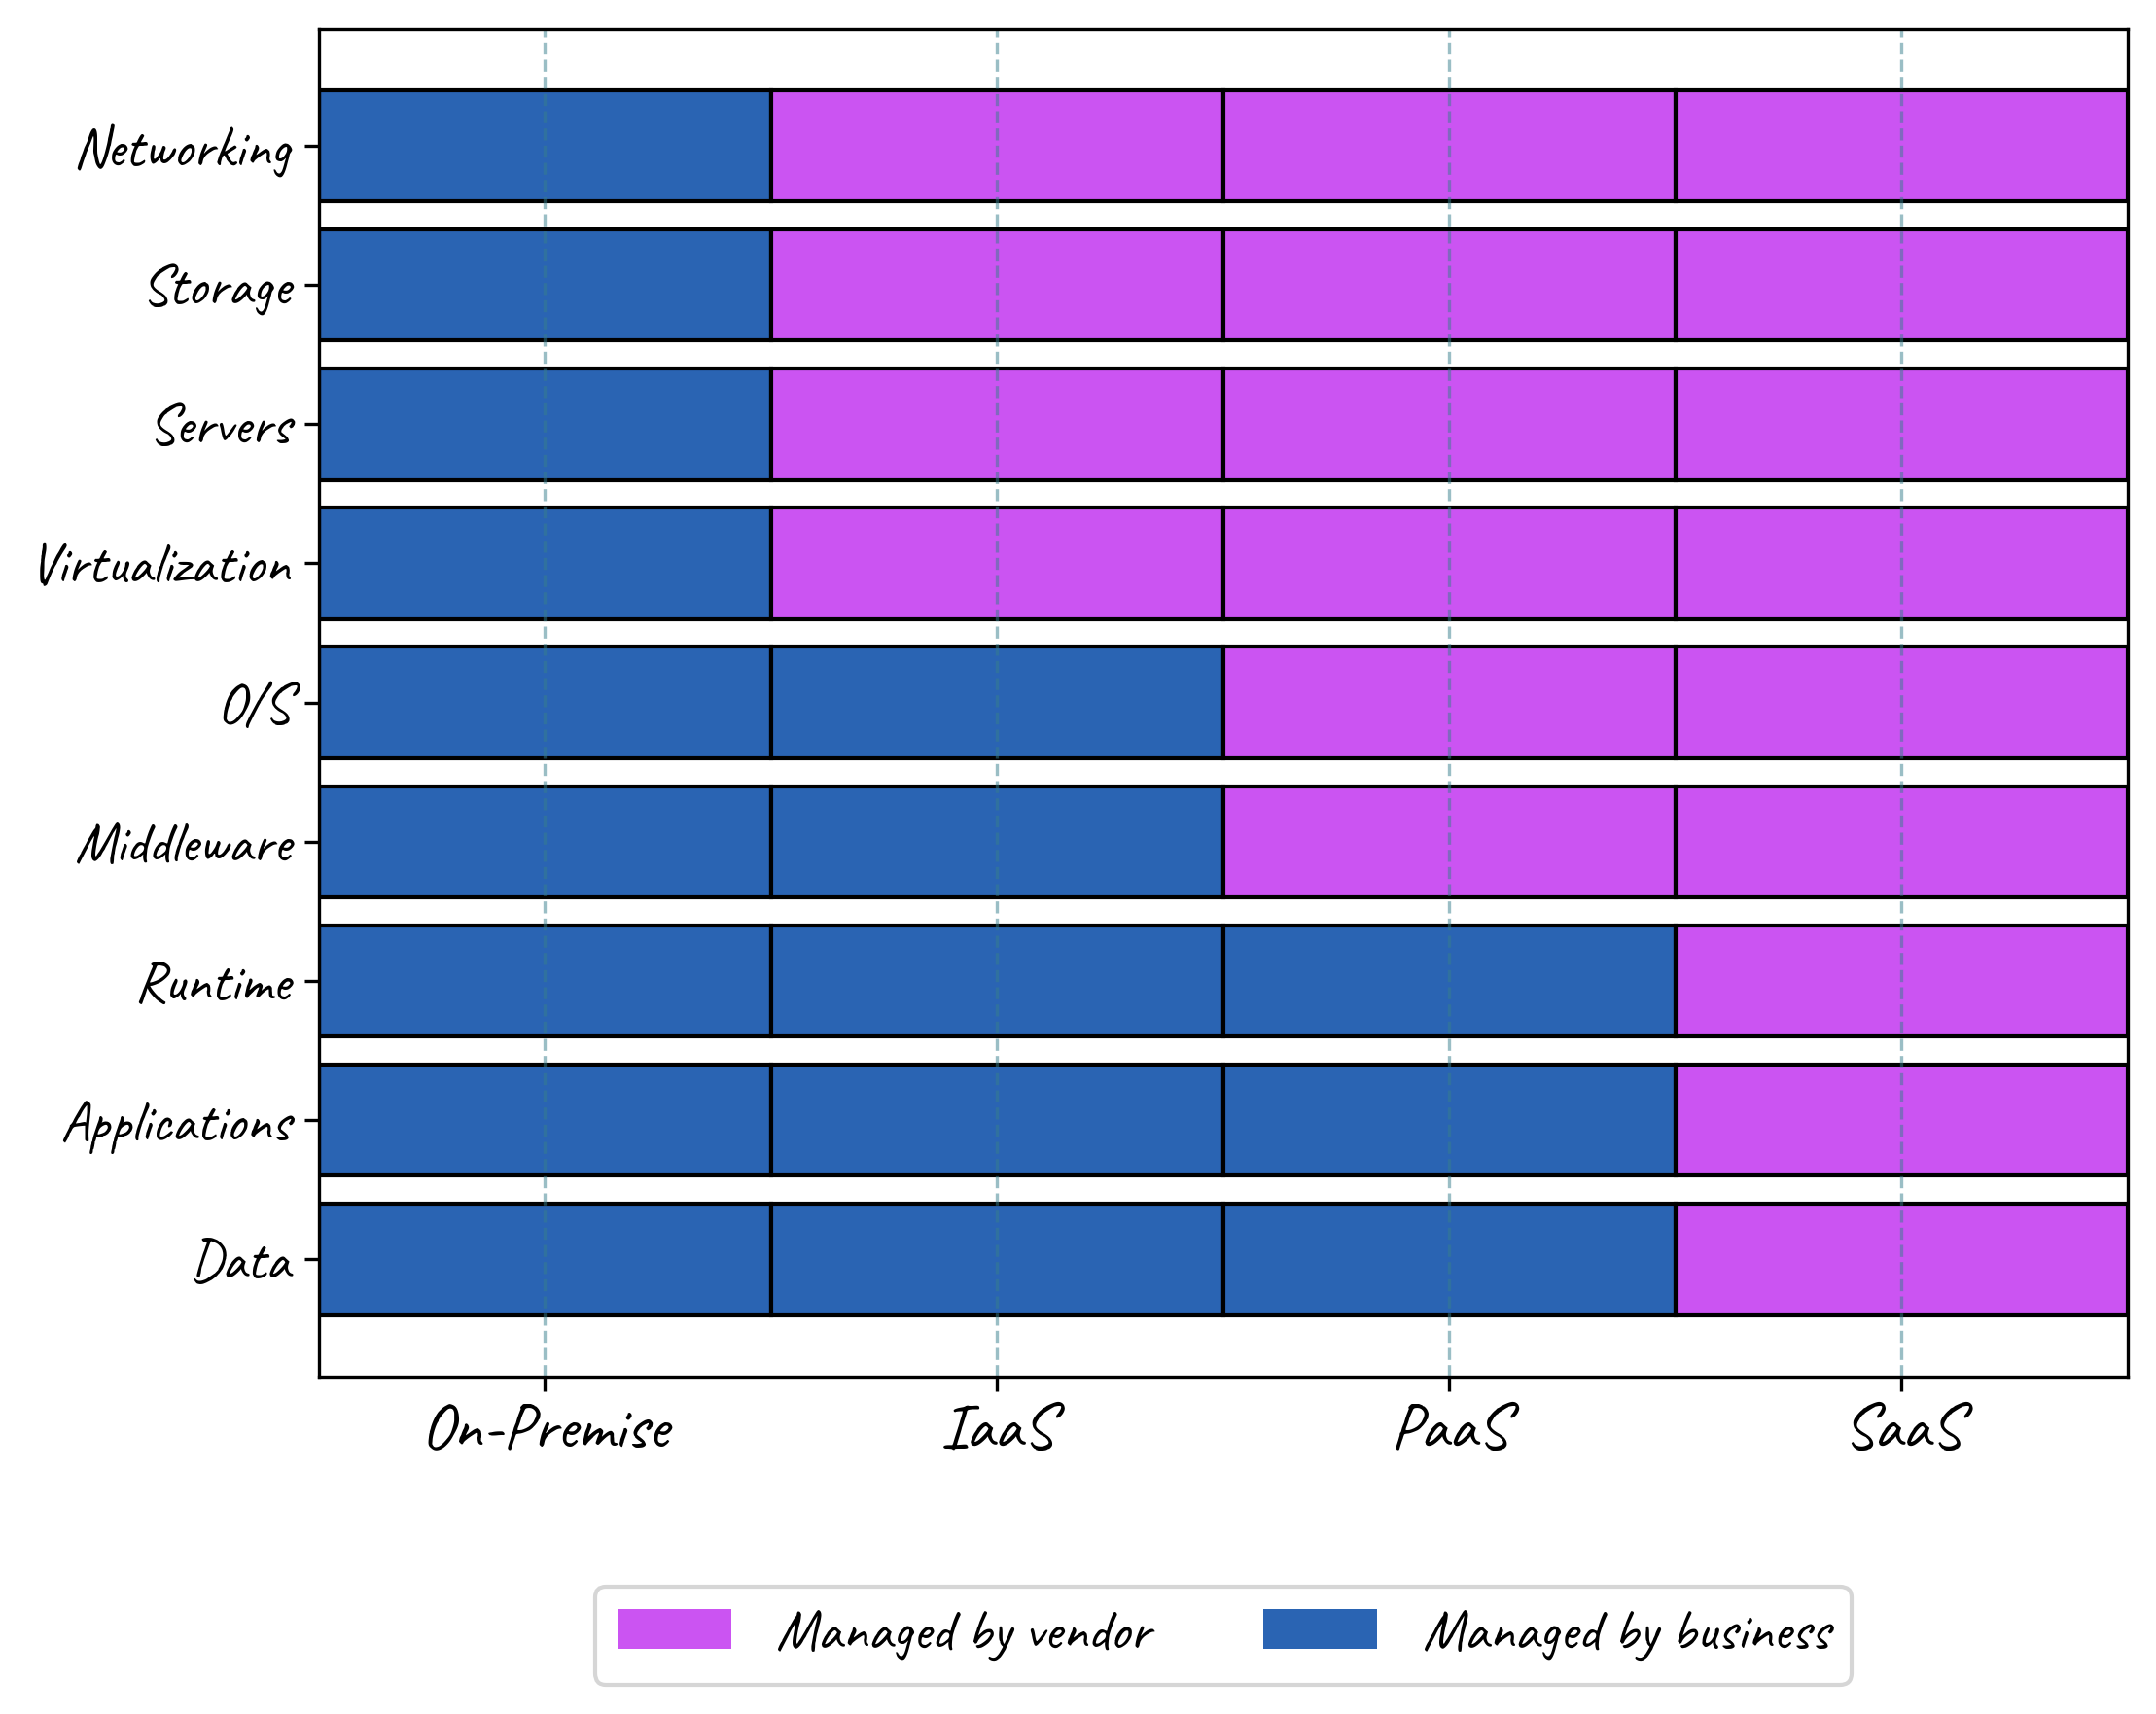
\includegraphics[width=0.8\textwidth]{infrastructure-models.png}
    \caption{Infrastructure models}
\end{figure}

\subsection{Observability and Monitoring}

Monitoring provides visibility into system health. Key components include:

\begin{itemize}
    \item \textbf{Metrics:} Measuring CPU, memory, latency.
    \item \textbf{Logging:} Centralized log aggregation (e.g., ELK stack).
    \item \textbf{Tracing:} Distributed tracing for debugging microservices.
\end{itemize}

\subsection{Incident Management and Reliability}

A structured approach to incident management is essential for maintaining system reliability and ensuring business continuity. As organisations increasingly depend on technology, a well-defined incident response process mitigates downtime, enhances resilience, and fosters continuous improvement.

\subsubsection{Incident Response Plan}

An effective incident response plan (IRP) provides predefined escalation paths, roles, and procedures that guide the organisation during a crisis. A comprehensive IRP typically includes the following key elements:

\begin{itemize}
    \item \textbf{Detection and Identification:} Implementing monitoring tools such as Prometheus, Datadog, or AWS CloudWatch to detect anomalies and trigger alerts.
    \item \textbf{Classification and Prioritisation:} Categorising incidents based on severity levels (e.g., P1, P2, P3) to ensure a proportionate response.
    \item \textbf{Escalation and Communication:} Defining communication protocols and using tools like PagerDuty or Slack to alert on-call engineers and stakeholders.
    \item \textbf{Resolution and Mitigation:} Applying predefined playbooks and automated remediation mechanisms to reduce mean time to resolution (MTTR).
    \item \textbf{Review and Documentation:} Capturing key incident details to inform future prevention strategies.
\end{itemize}

A well-structured IRP reduces confusion during crises and accelerates recovery, ensuring minimal impact on users and business operations.

\subsubsection{Postmortems and Continuous Learning}

Postmortems are essential for learning from past failures and improving reliability over time. A blameless postmortem culture fosters transparency and accountability while encouraging proactive risk mitigation. Key components of an effective postmortem include:

\begin{enumerate}
    \item \textbf{Incident Summary:} A clear description of the event, impact, and affected systems.
    \item \textbf{Root Cause Analysis (RCA):} Identification of underlying factors, often using methodologies such as the "Five Whys" or Fishbone Diagrams.
    \item \textbf{Timeline of Events:} A chronological breakdown of detection, response, and resolution actions.
    \item \textbf{Lessons Learned:} Insights gained from the incident, highlighting gaps in monitoring, automation, or communication.
    \item \textbf{Action Items:} Concrete steps to prevent recurrence, assigned to responsible teams with defined deadlines.
\end{enumerate}

Organisations such as Google and Netflix have adopted postmortem processes to enhance system reliability, demonstrating the effectiveness of continuous learning in technology operations \cite{allspaw2012postmortem}.

\subsubsection{Redundancy and High Availability}

Ensuring system reliability requires designing for failure through redundancy and high availability. This involves implementing fault-tolerant architectures that can withstand component failures without significant service degradation. Key strategies include:

\begin{table}[h]
    \centering
    \begin{tabular}{|l|p{10cm}|}
        \hline
        \textbf{Strategy}       & \textbf{Description}                                                                                      \\
        \hline
        Load Balancing          & Distributing traffic across multiple servers using tools like AWS ELB, Nginx, or HAProxy.                 \\
        \hline
        Database Replication    & Using primary-replica setups or multi-region replication in databases like PostgreSQL, MySQL, or MongoDB. \\
        \hline
        Multi-Cloud Deployments & Running services across multiple cloud providers (e.g., AWS and GCP) to mitigate cloud outages.           \\
        \hline
        Auto-Healing Mechanisms & Implementing self-healing infrastructure using Kubernetes, Terraform, or AWS Auto Scaling Groups.         \\
        \hline
        Disaster Recovery (DR)  & Establishing backup strategies, warm/cold failover plans, and automated recovery drills.                  \\
        \hline
    \end{tabular}
    \caption{Redundancy and High Availability Strategies}
    \label{tab:redundancy-strategies}
\end{table}

These redundancy techniques enhance fault tolerance and ensure seamless user experiences even in the face of unexpected failures.

\subsubsection{Conclusion}

A robust incident management and reliability strategy is integral to building scalable, resilient technology. By implementing structured incident response plans, fostering a blameless postmortem culture, and designing for redundancy, organisations can minimise downtime and enhance service reliability. These best practices ultimately contribute to sustained business growth and customer trust.

\bibliographystyle{plain}
\begin{thebibliography}{9}
    \bibitem{allspaw2012postmortem} Allspaw, J. (2012). \textit{Postmortem Culture: Learning from Failure}. Velocity Conference.
\end{thebibliography}



\bibliographystyle{plain}

\begin{thebibliography}{9}
    \bibitem{allspaw2012postmortem} Allspaw, J. (2012). \textit{Postmortem Culture: Learning from Failure}. Velocity Conference.
\end{thebibliography}



\chapter{Conclusion: Evolving as a CTO}

\section{The Ever-Changing Tech Landscape}

The role of a CTO is defined by continuous change. Technology is evolving at an unprecedented rate, impacting industries, business models, and leadership strategies. A CTO must remain vigilant, monitoring shifts in technology and adjusting strategies accordingly.

\subsection{Key Trends Influencing the CTO Role}

Some of the most significant trends that shape the modern CTO include:

\begin{itemize}
    \item \textbf{Cloud Computing and Edge Computing} - Increasing adoption of cloud platforms and the emergence of edge computing for real-time processing.
    \item \textbf{Artificial Intelligence and Machine Learning} - The rapid advancement of AI is transforming decision-making, automation, and customer interactions.
    \item \textbf{Cybersecurity} - Rising threats require CTOs to prioritize security strategies, governance, and compliance frameworks.
    \item \textbf{Quantum Computing} - Although still in its early stages, quantum computing holds the potential to revolutionize data processing and encryption.
    \item \textbf{Remote Work and Digital Collaboration} - New workforce trends demand secure, efficient, and scalable remote collaboration tools.
\end{itemize}

\subsection{Strategic Responses to Change}

A successful CTO must anticipate and respond to these trends with a proactive strategy. The following table outlines key challenges and potential responses:

\begin{table}[ht]
    \centering
    \begin{tabular}{|p{5cm}|p{10cm}|}
        \hline
        \textbf{Challenge}               & \textbf{Strategic Response}                                                                          \\
        \hline
        Rapid technological advancements & Invest in continuous learning, attend industry events, and foster a culture of innovation.           \\
        \hline
        Increasing cybersecurity threats & Implement zero-trust security models, perform regular audits, and educate teams on best practices.   \\
        \hline
        Workforce transformation         & Adopt flexible work models, invest in digital collaboration tools, and focus on employee experience. \\
        \hline
        Regulatory changes               & Stay informed on compliance requirements and work closely with legal and compliance teams.           \\
        \hline
    \end{tabular}
    \caption{CTO Challenges and Strategic Responses}
\end{table}

\section{Lifelong Learning and Adaptability}

To stay relevant as a CTO, continuous learning is not optional \textemdash{} it is a necessity. The following approaches can help CTOs maintain a competitive edge:

\subsection{Learning Channels for CTOs}

\begin{itemize}
    \item \textbf{Books and Research Papers} - Staying updated with foundational knowledge and emerging theories.
    \item \textbf{Industry Conferences and Webinars} - Learning from thought leaders and networking with peers.
    \item \textbf{Technical Courses and Certifications} - Ensuring hands-on expertise in relevant technologies.
    \item \textbf{Engaging with Developer Communities} - Gaining insights from grassroots innovations and developer feedback.
    \item \textbf{Experimentation and Prototyping} - Testing emerging technologies within a controlled environment.
\end{itemize}

\subsection{Developing an Adaptive Mindset}

Adaptability is not just about learning new skills but also about embracing change. A CTO must:

\begin{itemize}
    \item Foster a culture of experimentation within their teams.
    \item Encourage feedback loops for iterative improvement.
    \item Stay open to new methodologies, such as Agile, DevOps, and Lean principles.
    \item Maintain a balance between long-term strategy and short-term tactical changes.
\end{itemize}

\section{Final Thoughts and Next Steps}

The journey of a CTO is one of perpetual evolution. Mastery in technology leadership is not about reaching a final destination but about continuous improvement.

\subsection{Key Takeaways}

\begin{itemize}
    \item The CTO must be a strategic leader, not just a technical expert.
    \item Understanding and responding to technology trends is critical to success.
    \item Lifelong learning and adaptability are essential for long-term relevance.
    \item A CTO must balance innovation with stability and security.
    \item Building strong relationships with other C-suite executives enhances business impact.
\end{itemize}

\subsection{Next Steps for CTOs}

For those looking to refine their skills and impact, consider the following actionable steps:

\begin{enumerate}
    \item \textbf{Conduct a self-assessment} - Identify strengths and areas for improvement.
    \item \textbf{Set learning goals} - Commit to gaining expertise in one emerging technology each year.
    \item \textbf{Expand your professional network} - Engage with mentors, industry leaders, and communities.
    \item \textbf{Experiment with new technologies} - Implement pilot projects to understand new tools firsthand.
    \item \textbf{Develop a legacy plan} - Focus on long-term contributions and preparing the next generation of leaders.
\end{enumerate}

By embracing these principles and steps, a CTO can ensure they remain at the forefront of technological leadership, ready to guide their organization through the challenges and opportunities of an ever-evolving digital landscape.

\backmatter

\appendix
\section*{Book creation details}

This book was created using \LaTeX{} and hosted on GitHub. The workflow includes managing issues and pull requests to facilitate collaboration.

\subsection*{Creative Commons License}

This book is distributed under the Creative Commons Attribution-ShareAlike 4.0 International License. This license allows you to share and adapt the content as long as you attribute the author and share your contributions under the same license.

\section*{About the Author}

Santiago Lizardo is a technical leader with over 20 years of experience in the technology industry. He studied computing, mathematics, and statistics and has dedicated his most recent years to deepening his knowledge in leadership and management.

His extensive professional experience includes roles as CTO, software architect, and development team leader, where he has worked on defining and executing technological strategies for companies of various sizes and sectors.

He was the founder of two tech startups and has led development teams in software companies in Argentina, Spain, and the United Kingdom.

Currently, he serves as the Head of Engineering at a hardware and software company with a presence in the United Kingdom and the United States, where he applies the principles and practices presented in this book.


\listoffigures
\listoftables
% \lstlistoflistings

\clearpage
\printindex

\end{document}
